L'objectif de l'analyseur sémantique est l'interprétation pure et simple de l'arbre abstrait précédement généré. En effet, le but ici est l'exécution du code écrit en Stibbons, et l'interprète prend ainsi en paramètre un arbre ainsi qu'un agent sur lequel exécuté cet arbre, et effectue un parcours en profondeur de l'arbre, se rappelant récursivement sur chaque nœud fils de l'arbre. 

\subsection{Fonctionnement}
Lors de l'analyse d'un jeton, qui correspond à un nœud de l'arbre syntaxique, on analyse d'abord ses fils (s'il y en a) puis ensuite le contenu du noeud courant.
Par exemple, pour le test d'égalité \verb|1 == 2|, le nœud \verb|<EQ>| aura pour enfants les sous-arbres \verb|<NUMBER,1>| et \verb|<NUMBER,2>|. Ces deux derniers seront interprétés en premier et renverront leurs valeurs sémantiques (en l'occurence, des \verb|stibbons::Number| ayant respectivement pour valeur 1 et 2), puis le test \verb|==| sera appliqué sur ces résultats.

Nous avons dû faire un certain nombre de choix sémantique lors de l'élaboration de notre langage, et en voici quelques uns particuliers~:
\begin{description}
\item[affectation] Lors d'une affectation, on modifie en priorité les paramètres de l'agent ou de la fonction courante, si l'identifiant existe dans la table des paramètres, sinon, on modifie la propriété correspondante de l'agent.
\item[identifiant] Lorsque l'on accède à la valeur d'un identifiant, on recherche tout d'abord cet identifiant dans les paramètres de l'agent courant. S'il n'existe pas, on le recherche dans les propriétés de l'agent courant. Ainsi, la portée des «~variables~» est exclusivement locale à l'agent. On peut explicitement accéder à une propriété d'un autre agent, via l'opérateur «~.~».
\item[fonction] les fonctions sont des valeurs. Ainsi, tout comme les valeurs, leurs créations a un comportement similaire à une affectation et leur accès également (espace de noms des fonctions et des variables communs).
\item[agent] la création d'un nouveau type agent, où qu'elle soit faite, est liée au monde et est, par conséquent, accessible depuis tous les agents.
\end{description}

\subsection{Fonctionnalités}

\subsubsection{Sprints 1 et 2}
Les deux premiers sprints ont été assez conséquent au niveau du nombre de fonctionnalités ajoutées.
En effet lors du sprint 1, on pouvait déjà effectuer les opérations de bases sur une tortue, telles que avancer, tourner, écrire, etc. De plus les opérations de calcul ainsi que la gestion de nombres ont été fait. En effet, il était nécessaire de gérer les nombres de manière à pouvoir indiquer à la tortue de quelle distance elle devait avancer.

Lors du deuxième sprint sont apparu les conditionnelles, ainsi que les boucles, les comparaisons binaires, les booléens et autres types (color, string, etc.), la création de nouveaux agents dans le code et les fonctions sans paramètres. Ce sprint fut alors une version déjà bien avancée de notre programme final.

\subsubsection{Sprint 3 à 5}
Les sprints suivants ont été plus léger. Non pas parce qu'il y avait moins de travail, car la gestion de l'interpréteur fut remanier à ce moment là, mais car il y avait moins de fonctionnalités à ajouter. En effet, à partir du sprint 3, les fonctionnalités suivantes ont été rajoutés~:
\begin{itemize}
\item accès à la parenté et aux zones~;
\item ajout des tables et de boucles dédiés (\verb|foreach|)~;
\item gestion de la vitesse et de la pause~;
\item ajout des communications avec le \verb|send| et le \verb|recv|.
\end{itemize}

\subsection{Organisation}

L'analyseur sémantique a d'abord été une seule classe~: la classe \verb|Interpreter|.
Cette dernière implémentait tout types d'actions à effectuer pour n'importe quel type d'agent.
Cependant, lors de l'arrivée de la fonctionnalité d'ajout d'un nouvel agent (\verb|new agent|), nous nous sommes aperçu qu'il serait mieux d'avoir un interpréteur par type d'agent, ou plus précisement un interpréteur pour le monde, un pour les tortues et un pour les actions communes aux deux types (cf. UML~\ref{interpreterUML}).
Nous avons alors crée les deux classes~: \verb|WorldInterpreter| et \verb|TurtleInterpreter|.

Ainsi, par exemple, si on demande à une tortue d'avancer en Stibbons (\verb|fd 10|), alors c'est le \verb|TurtleInterpreter| qui gèrera cette action.
A contrario, si on effectue une affectation (ex : \verb|a = 10|) alors l'\verb|Interpreter| affectera la valeur \verb|10| à la propriété \verb|a| de l'agent courant.

De manière parallèle, la création du monde s'effectuait dans l'\verb|Interpreter|, puis dans le \verb|WorldInterpreter|, il fut alors nécessaire de créer une classe qui gérerait à la fois la création du monde et tout ce qui concernait l'application (la pause, le temps, les interpreteurs eux-mêmes). Nous avons alors décidé de créer la classe \verb|InterpreterManager|.
Cette classe connait tous les interpréteurs, et permet de les prévenir d'une éventuelle pause du programme, de stocker les threads correspondants à chaque interpréteur, de créer un monde avec les pré-directives choisies~; c'est une sorte de gestionnaire d'interpréteurs.

\begin{figure}[h]
\caption{\label{interpreterUML} UML de l'analyseur sémantique}
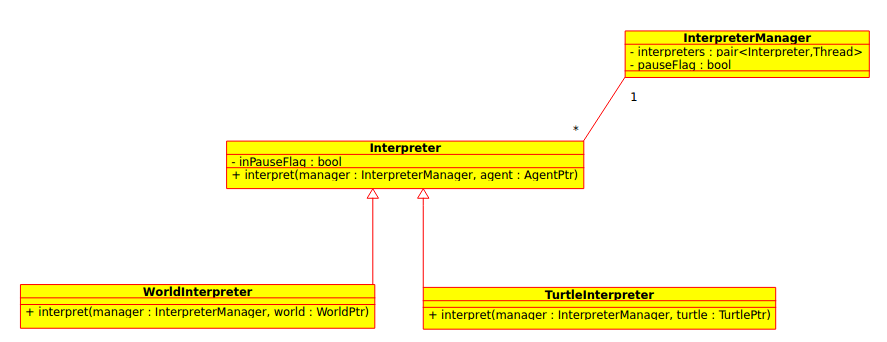
\includegraphics[scale=0.5]{doc/report/uml/interpreterUML.png}
\end{figure}
